\documentclass[a4paper]{ctexart}

\usepackage{tabularx} % extra features for tabular environment
\usepackage{amsmath}  % improve math presentation
\usepackage{graphicx} % takes care of graphic including machinery
\usepackage[margin=1in,letterpaper]{geometry} % decreases margins
\usepackage{cite} % takes care of citations
\usepackage[final]{hyperref} % adds hyper links inside the generated pdf file
\usepackage{ctex}
\usepackage{titlesec}
%\usepackage{CJKutf8, CJK}
\usepackage{makecell}                 % 三线表-竖线
\usepackage{booktabs}                 % 三线表-短细横线
% \usepackage{natbib}
\usepackage{graphicx}				  % 表格单元格逆时针
\usepackage{multirow}				  % 合并单元格
\usepackage{array}
\usepackage{amssymb}				  % 勾
\usepackage{amsmath}
\usepackage{longtable}                % 导入 longtable 宏包,表格自动换行
\usepackage{caption}
\usepackage{subcaption}               % 设置子图
\usepackage{caption}
%\usepackage{subfigure}
\usepackage{diagbox}
\usepackage{color}					  % 文本颜色包
\usepackage{colortbl}
\usepackage{xcolor}
\usepackage{bbm}					  % 输入指示函数
\usepackage{tablefootnote}			  % 表格注释
\usepackage{pythonhighlight}
%\usepackage{fancyhdr}
\usepackage{lastpage}
\usepackage{tocloft}
\usepackage{authblk}
\usepackage{setspace}
\usepackage{float}
\usepackage[section]{placeins}

% 设置页面边距
\geometry{a4paper, top=1.7cm, bottom=1.6cm, left=1.6cm, right=1.6cm}

%\pagestyle{fancy}
%\fancyhf{}
%\fancyhead{}
%\fancyfoot{}
%\fancyhead[R]{\small Page \thepage\ of \pageref*{LastPage}}
%\fancyhead[L]{\zihao{-5} \songti 开题报告}

\usepackage{listings}                 % 导入代码块
\usepackage{xcolor}

% 定义适合黑色背景的配色方案
\definecolor{vscodeblue}{RGB}{97, 175, 239}  % keywords
\definecolor{vscodegreen}{RGB}{152, 195, 121}% comments
\definecolor{vscodepurple}{RGB}{198, 120, 221}% strings
\definecolor{vscodegray}{RGB}{153,153,153}   % line numbers
\definecolor{vscodeorange}{RGB}{224,108,117} % function names
\definecolor{vscodebackground}{RGB}{40,44,52} % 黑色背景
\definecolor{vscodewhite}{RGB}{248,248,242}  % 白色字体

% 设置 C++ 代码块的样式,适合黑色背景
\lstset{
	language=C++,
	backgroundcolor=\color{vscodebackground},  % 黑色背景
	basicstyle=\ttfamily\footnotesize\color{vscodewhite}, % 白色文字,紧凑的字体大小
	keywordstyle=\color{vscodeblue}\bfseries,  % 关键字颜色
	commentstyle=\color{vscodegreen}\itshape,  % 注释颜色
	stringstyle=\color{vscodepurple},          % 字符串颜色
	numberstyle=\tiny\color{vscodegray},       % 行号颜色
	numbers=left,                              % 行号显示在左侧
	stepnumber=1,                              % 每行都显示行号
	numbersep=5pt,                             % 行号与代码之间的距离
	tabsize=4,                                 % tab 键宽度
	showspaces=false,                          % 不显示空格符号
	showstringspaces=false,                    % 字符串中的空格不显示特殊符号
	breaklines=true,                           % 自动换行
	breakatwhitespace=true,                    % 只在空格处换行
	columns=fullflexible,                      % 紧凑的代码对齐
	keepspaces=true,                           % 保持空格符号
	frame=single,                              % 给代码块加框
	framesep=3pt,                              % 代码与框之间的距离
	rulecolor=\color{vscodegray},              % 框的颜色
	escapeinside={(*@}{@*)},                   % 允许LaTeX注释
	xleftmargin=10pt,                          % 左边距
	xrightmargin=10pt,                         % 右边距
}

\hypersetup{
	colorlinks=true,       % false: boxed links; true: colored links
	linkcolor=blue,        % color of internal links
	citecolor=blue,        % color of links to bibliography
	filecolor=magenta,     % color of file links
	urlcolor=blue         
}
%++++++++++++++++++++++++++++++++++++++++
\titleformat{\section}{\Large\bfseries}{\thesection}{1em}{}
\titleformat{\subsection}{\large\bfseries}{\thesubsection}{1em}{}
\titleformat{\subsubsection}{\normalsize\bfseries}{\thesubsubsection}{1em}{}
\titleformat{\paragraph}[runin]{\normalsize\bfseries}{\paragraph}{1em}{}
\titleformat{\subparagraph}[runin]{\normalsize\bfseries}{\subparagraph}{1em}{}

\begin{document}
	
\section{二叉树消消乐}
	
\begin{center}
	\Large \textbf{二叉树消消乐}
\end{center}
	
\noindent\textbf{时间限制:} \textbf{C/C\texttt{++}} 1000ms,其他语言:2000ms

\noindent\textbf{内存限制:} \textbf{C/C\texttt{++}} 256MB,其他语言:512MB
	
\vspace{10pt}
	
\noindent\textbf{题目描述:}
	
给定原始二叉树和参照二叉树(输入的二叉树均为满二叉树,二叉树节点的值范围为[1,1000],二叉树的深度不超过1000),现对原始二叉树和参照二叉树中相同层级目值相同的节点进行消除,消除规则为原始二叉树和参照二叉树中存在多个值相同的节点只能消除等数量的,消除后的节点变为无效节点,请按节点值出现频率从高到低输出消除后原始二叉树中有效节点的值(如果原始二叉树消除后没有有效节点返回0)。
	
\noindent\textbf{输入描述:}
	
原始二叉树中的节点个数

原始二叉树

参照二叉树中的节点个数

参照二叉树
	
\noindent\textbf{输出描述:} 
	
原始二叉树中有效节点的值,按出现频率从高到低排序(相同频率的值按大小排序),相同频率的值按降序排列。
	
\noindent\textbf{样例输入1:}
	
\lstset{numbers=none}
\begin{lstlisting}
7
1 3 3 3 4 5 6
3
2 3 4
\end{lstlisting}
\lstset{numbers=left}
	
\noindent\textbf{样例输出1:}
\lstset{numbers=none}
\begin{lstlisting}
36541
\end{lstlisting}
\lstset{numbers=left}
	
\noindent 样例 1 解释:原始二叉树 A 消除参照二叉树 B 中的重复元素后,有效节点剩余 2 个 3,1 个 6,1 个 5,1 个 4,1 个 1,3 出现的频率 2, 6、5、4、1 出现的频率为 1,按值从大到小排序,所以排序结果为 36541。

\noindent\textbf{样例输入2:}
\lstset{numbers=none}
\begin{lstlisting}
15
5 6 6 6 7 7 7 8 8 9 9 7 7 5 6
7
5 6 6 7 7 8 8
\end{lstlisting}
\lstset{numbers=left}
	
\noindent\textbf{样例输出2:}
\lstset{numbers=none}
\begin{lstlisting}
79865
\end{lstlisting}
\lstset{numbers=left}

\noindent 样例 2 解释:原始二叉树 A 消除参照二叉树 B 中的重复元素后,有效节点剩余 3 个 7,2 个 9,2 个 8,2 个 6,1 个 5,8 出现的频率 3, 7 出现的频率为 2,6 出现的频率为 2,6 的值比 5 大,所以排序结果为 79865。
	
\vspace{10pt}
	
\noindent\textbf{思路分析:}
\begin{itemize}
	\item [1.] \textbf{按照题目要求构建二叉树} 
	
	\item [2.] \textbf{统计参照二叉树每一层节点的出现次数,这一步可以使用哈希表来完成}
	
	\item [3.] \textbf{遍历原始二叉树,每一层的节点减去当前参照二叉树的对应节点的值的数量即可}
\end{itemize}

\noindent\textbf{难点分析:}
\begin{itemize}
	\item [1.] \textbf{二叉树的层次遍历(BFS)}
	
	每层的结点需要进行单独的处理和统计,这意味着遍历时要保存当前节点以及下一层节点,这通常使用队列 \texttt{queue} 来完成。
	
	\item [2.] \textbf{如何在遍历原始树时根据参照树减少节点数量}
	
	需要对比原始二叉树和参照二叉树中每层的节点,并且根据参照树中的节点数来更新原始树的节点频率。这一部分需要巧妙地通过哈希表来存储每层节点的出现次数,然后在遍历原始树时进行相应的扣减。
	
	\item [3.] \textbf{频率和节点值的排序}
	
	在节点删除和频率统计完成之后,需要对剩下的有效节点进行排序。
	
\end{itemize}

\noindent\textbf{实现代码:}
	
\begin{lstlisting}
#include <iostream>
#include <vector>
#include <queue>
#include <unordered_map>
#include <algorithm>

using namespace std;

int main() { 
	int n, m;
	cin >> n;
	
	vector<int> nums1(n);
	for (int i = 0; i < n; ++i) { 
		cin >> nums1[i];
	}
	
	cin >> m;
	vector<int> nums2(m);
	for (int i = 0; i < m; ++i) { 
		cin >> nums2[i];
	}
	
	// 定义一个二维哈希表,用于统计参照二叉树每层结点的出现次数
	vector<unordered_map<int, int>> nums2_cnt(1001);
	queue<int> q; // 用于层序遍历的队列
	
	q.push(0); // 根结点的层号为 0
	int depth = 0; // 当前结点的深度
	
	// 统计参照二叉树每层结点的出现次数
	while (!q.empty()) { 
		int length = q.size(); // 当前层的结点个数
		for (int i = 0; i < length; ++i) { 
			int node = q.front(); // 取队首元素
			q.pop(); // 出队
			nums2_cnt[depth][nums2[node]]++; // 当前结点的出现次数加 1
			if (node * 2 + 1 < m) { 
				q.push(node * 2 + 1); // 左孩子入队
				q.push(node * 2 + 2); // 右孩子入队
			}
		}
		depth++;
	}
	
	// 使用哈希表统计原始二叉树的结点出现次数
	unordered_map<int, int> nums1_cnt;
	for (int num : nums1) {
		nums1_cnt[num]++; 
	}
	
	// 遍历原始二叉树,逐层处理并减去参照树对应层的结点
	q.push(0); // 根结点的层号为 0
	depth = 0; // 当前结点的深度
	
	while (!q.empty()) {
		int length = q.size();
		unordered_map<int, int> cur; // 临时哈希表,用于存储当前层结点的出现次数
		
		for (int i = 0; i < length; ++i) { 
			int node = q.front(); // 取队首元素
			q.pop(); // 出队
			cur[nums1[node]]++; // 当前结点的出现次数加 1
			if (node * 2 + 1 < n) { 
				q.push(node * 2 + 1); // 左孩子入队
				q.push(node * 2 + 2); // 右孩子入队
			}
		}
		
		for (auto &kv : cur) { 
			int k = kv.first;
			int v = kv.second;
			if (nums2_cnt[depth][k] >= 0) { 
				nums1_cnt[k] = max(nums1_cnt[k] - nums2_cnt[depth][k], 0); // 减去参照树对应层的结点
			}
		}
		depth++;
	}
	
	vector<pair<int, int>> sorted_dic(nums1_cnt.begin(), nums1_cnt.end());
	sort(sorted_dic.begin(), sorted_dic.end(), [](const pair<int, int> &a, const pair<int, int> &b) { 
		if (a.second != b.second)
		return a.second > b.second;
		return a.first > b.first;
	});
	
	// 输出结果
	for (auto &p : sorted_dic) {
		if (p.second > 0)
		cout << p.first;
	}
	cout << endl;
	
	return 0;
}
\end{lstlisting}
	
\newpage
	
\section{好友推荐系统}
	
\begin{center}
	\Large \textbf{好友推荐系统}
\end{center}
	
\noindent\textbf{时间限制:} \textbf{C/C\texttt{++}} 1000ms,其他语言:2000ms
	
\noindent\textbf{内存限制:} \textbf{C/C\texttt{++}} 256MB,其他语言:512MB
	
\vspace{10pt}
	
\noindent\textbf{题目描述:}
	
你正在为一个社交网络平台开发好友推荐功能。

平台上有N个用户(每个用户使用1到 N的整数编号),同时系统中维护了用户之间的好友关系。

为了推荐新朋友,平台决定采用“共同好友数量"作为衡量两个用户之间相似度的标准。

系统根据输入用户编号K,输出与此用户K相似度最高的前L个用户ID,来推荐给用户K

\textit{相似度定义:两个用户非好友,两个用户的相似度为拥有的共同好友数(例如用户A和用户B,只有共同好友C和D,相似度=2)}
	
\noindent\textbf{输入描述:}
	
第一行包含四个整数 N,M、K 和 L,分别表示用户的数量(N),好友记录条数(M)、查询的用户编号(K)和推荐的好友数量(L)。
	
接下来 M 行,每行包含两个整数编号 X 和 Y,表示编号为 X 和 Y 用户是好友。

1) 输入格式都是标准的,无需考虑输出异常场景(不会包含用户和自己是好友的输入,例如 1 1)

2) 用户数不超过 1024

3) 好友记录数不超过10240
	
\noindent\textbf{输出描述:} 
	
根据输入 K 和 L,输出和用户 K 相似度最高的 L 个用户编码。

1) 输出相似度最高的前 L 个用户编码,按照相似度从高到低排序;

2) 如果有相似度相同的可能好友,按照用户编号从小到大排序;

3) 如果推荐的好友个数不足 L 个,则推荐与用户 K \textbf{无共同好友关系}的用户(陌生人)作为可能好友;如果推荐仍不满足 L 个用户,剩余推荐用户编码使用 0 来占位。
	
\noindent\textbf{样例输入1:}
	
\lstset{numbers=none}
\begin{lstlisting}
6 7 3 2
1 2
1 3
2 3
3 4
3 5
4 5
5 6
\end{lstlisting}
\lstset{numbers=left}
	
\noindent\textbf{样例输出1:}
\lstset{numbers=none}
\begin{lstlisting}
6 0
\end{lstlisting}
\lstset{numbers=left}

\noindent 样例1解释:

输入包含了6个用户,7条好友记录,给用户ID编号为3的用户推荐2个好友。

输出只有编号为6的用户可能是编号3用户的可能好友;

尝试推荐与编号3用户无共同好友的其他用户,由于除编号为6的用户之外,其他用户和编号3用户都是好友,所以找不到陌生人作为推荐的第二个用户:推荐结果不足2个用户,所以推荐的第二个用户编码使用0来占位补足。

\noindent\textbf{样例输入2:}

\lstset{numbers=none}
\begin{lstlisting}
8 11 1 3
1 2
1 3
2 3
3 4
3 5
4 5
5 6
6 7
7 8
1 8
2 7
\end{lstlisting}
\lstset{numbers=left}

\noindent\textbf{样例输出2:}
\lstset{numbers=none}
\begin{lstlisting}
7 4 5
\end{lstlisting}
\lstset{numbers=left}
	
\noindent 样例2解释:

输入包含了8个用户,11条好友记录,给用户ID编号为1的用户推荐3个好友。

按照相似度排序推荐给用户1的相关好友:7 4 5
	
\vspace{10pt}
	
\noindent\textbf{思路分析:}

\begin{itemize}
	\item [1.] \textbf{相似度计算} 
		相似度衡量两个用户是否有共同好友。推荐好友时,优先推荐相似度高的用户。如果两个用户的相似度相同,则推荐编号较小的用户。
		
	\item [2.] \textbf{特殊情况处理}
		\begin{itemize}
			\item[$\bullet$] 如果用户没有好友,则不会推荐好友;
			\item[$\bullet$] 如果没有足够的用户进行推荐,需要补充陌生人,最后补充0。
		\end{itemize}
\end{itemize}

\noindent\textbf{难点分析:}
\begin{itemize}
	\item [1.] \textbf{数据结构的选择和使用} 
	
	题目中涉及用户与用户之间的好友关系,这其实是一个图的建模问题。我们需要用适合的方式来存储每个用户及其好友的关系。这里选择了邻接表 \texttt{vector<set<int>> friends} 来存储用户之间的好友关系,每个用户的好友使用 \texttt{set} 存储,以便能够快速查找、插入和删除好友信息。
	
	\textbf{难点}:如果不熟悉图的表示方法以及如何选择合适的数据结构(如邻接矩阵或邻接表),可能会在存储和查找好友关系上遇到问题。
	
	\item [2.] \textbf{相似度计算逻辑}
	
	题目要求推荐相似度高的用户,具体的标准是与目标用户 K 有共同好友的用户。遍历目标用户 K 的所有好友后,还需要继续遍历这些好友的好友,找出哪些用户与目标用户有共同好友。
	
	\textbf{难点}:这里的相似度计算涉及两层嵌套的循环,逻辑上容易出错。如果不仔细设计,可能会忽略掉一些潜在的推荐对象,或者误算一些用户的相似度。
	
	\item [3.] \textbf{排序规则的处理}
	
	按照相似度排序,处理相似度相同的情况:对于找到的潜在好友,需要按相似度从高到低排序。如果相似度相同,则按照用户 ID 进行升序排序。这涉及自定义排序规则的设计和实现。
	
	\textbf{难点}:自定义排序逻辑涉及到多个条件的判断,在实现过程中容易出错,比如优先级设置不当、排序不稳定等问题。
	
	\item [4.] \textbf{推荐数量不足的处理}
	
	补充非好友或空位:如果找到的潜在好友数量不足 L 个,还需要补充没有共同好友的非好友(即所谓的“陌生人”),如果仍然不足 L 个,则用 0 填补空位。这部分逻辑在实现上需要注意确保推荐结果的数量始终为 L,并且需要防止重复推荐。
	
	\textbf{难点}:如何优雅地处理“推荐不足 L 个”的情况,补充非好友并确保不重复推荐,设计这部分逻辑时需要严密的控制条件。
	
	\item [5.] \textbf{边界条件的处理}
	
	特殊情况:有一些特殊情况需要特别处理,比如目标用户 K 没有好友的情况,或者社交网络中总用户数 N 较少的情况。这些情况可能会导致潜在好友数量不足,需要特别处理以防止程序出错或产生不符合预期的输出。
	
	\textbf{难点}:边界条件的处理如果不仔细考虑,可能会导致错误的输出或程序崩溃。例如,处理目标用户没有好友的情况时,需要确保相似度计算不会发生。
	
\end{itemize}

\noindent\textbf{代码实现:}

1. \textbf{首先我们定义用户结构体 \texttt{User}}:

1) \texttt{User} 结构体定义了用户的编号 \texttt{id} 和相似度 \texttt{similarity}。

2) 定义自定义的排序规则:相似度高优先;如果相似度相同,编号较小的用户优先。

\begin{lstlisting}
/**
* User 结构体,用于存储用户编号和相似度
* 
* id                           表示用户的编号(ID),即社交网络中用户的唯一标识。
* similarity                   表示用户与用户K的相似度,即用户K的好友中有多少个是该用户的好友;
*                              相似度越高,表示他们有越多的共同好友。
* User(int id, int similarity) 含参构造函数,创建User对象时直接赋值给 id 和 similarity 这两个成员变量。
*                              User user(3, 5); 表示用户编号为3,与用户K的相似度为5。
* bool operator<(const User& other) const;               
*                              重载小于号运算符,用于自定义排序规则,相似度高优先,相似度相同时编号小优先。
*                              用于实现两个用户对象之间的比较,用于排序推荐好友列表。
*                              (const User& other) 表示传入的参数是一个 User 类型的对象。
*                              const         修饰函数,表示该函数不会修改成员变量的值。
*                              bool          返回值类型。
*                              return true   表示当前对象小于传入的对象。
*                              return false  表示当前对象大于传入的对象。
*/
struct User {
	int id, similarity;
	User(int id, int similarity) : id(id), similarity(similarity) {}
	// 自定义排序规则:相似度高优先,相似度相同时编号小优先
	bool operator<(const User& other) const {
		if (similarity == other.similarity)
		// 如果两个用户的相似度相同,选择 id 值较小的用户排在前面。
		return id < other.id;
		return similarity > other.similarity;
	}
};
\end{lstlisting}

2. \textbf{数据结构初始化和输入}

1) 在好友推荐系统中,我们可以使用邻接表来表示社交网络中的好友关系,社交网络中的用户可以被看作图中的顶点,用户之间的好友关系则被视为边。通过邻接表可以高效地存储和查找某个用户地好友列表,从而方便进行好友推荐、共同好友计算等操作。

2) 我们使用邻接表 \texttt{vector<set<int>> friends(N + 1);} 来存储每个用户的好友列表。我们通过遍历输入,构建每个用户的好友列表。

\begin{lstlisting}
/*
* 通过邻接表来构建图
* 1 -> 2 -> 3 -> 8
* 2 -> 1 -> 3 -> 7
* 3 -> 1 -> 2 -> 4 -> 5
* 4 -> 3 -> 5
* 5 -> 3 -> 4 -> 6
* 6 -> 5 -> 7
* 7 -> 6 -> 8 -> 2
* 8 -> 7 -> 1
*/
\end{lstlisting}

3. \textbf{计算用户 K 的潜在好友的相似度}

1) 我们需要计算用户 K 的潜在好友的相似度,通过一个哈希表 \texttt{unordered\_map<int, int> similarity;} 用于存储与用户 K 的相似度。

2) 我们遍历用户 K 的所有好友,在遍历这些好友的好友。对于每个不是 K 本身且不是 K 好友的用户,其相似度计数\texttt{+1}。

\begin{lstlisting}
/*
* unordered_map<int, int> similarity; 用于存储用户的好友关系。
* Key : Value
* 5 : 1
* 4 : 1
* 7 : 2
*/
\end{lstlisting}

4. \textbf{构建潜在好友列表并排序}

1) 我们构建潜在好友列表并排序,我们再遍历一遍所有用户,跳过 K 自己和 K 的现在好友;

2) 对每个用户构建 \texttt{User} 结构体,并存入 \texttt{potentialFriends};

3) 然后对潜在好友进行排序,排序的优先级是相似度高优先,相似度相同编号小优先。

\begin{lstlisting}
// 将结果放入一个用户结构体数组中
vector<User> potentialFriends;
for (int i = 1; i <= N; ++i) {
	if (i != K && !friends[K].count(i)) { // 不是自己且不是好友
		// 如果 similarity 中存在 i,则取出 i 的相似度,否则相似度为 0
		int sim = similarity.count(i) ? similarity[i] : 0; 
		// 将用户编号和相似度放入数组中
		potentialFriends.push_back(User(i, sim));
	}
}

// 对所有潜在好友进行排序
sort(potentialFriends.begin(), potentialFriends.end());
\end{lstlisting}

\begin{lstlisting}
/*
* User ID: 7, Similarity: 2
* User ID: 4, Similarity: 1
* User ID: 5, Similarity: 1
* User ID: 6, Similarity: 0
*/
\end{lstlisting}

5. \textbf{推荐好友并补充到 L 个}

1) 我们首先按照排序好的\texttt{potentialFriends}推荐好友,最多推荐 L 个;

2) 如果推荐不足 L 个,则补充没有共同好友的陌生人;

3) 如果仍然不足 L 个,则补充 0。

\begin{lstlisting}
vector<int> result;
int recommended = 0; // 记录已推荐的好友数量

// 按照相似度高低输出潜在好友
for (const User& user : potentialFriends) {
	if (recommended < L) {
		result.push_back(user.id);
		recommended++;
	} else {
		break;
	}
}

// 如果推荐不足L个,补充陌生人(没有与用户K共同好友的非好友)
for (int i = 1; i <= N && recommended < L; ++i) {
	if (i != K && !friends[K].count(i) && similarity.count(i) == 0) {
		if (find(result.begin(), result.end(), i) == result.end()) { // 避免重复推荐
			result.push_back(i);
			recommended++;
		}
	}
}

// 如果仍不足L个,补充0
while (recommended < L) {
	result.push_back(0);
	recommended++;
}
\end{lstlisting}

\noindent\textbf{完整代码:}
	
\begin{lstlisting}
#include <iostream>
#include <vector>
#include <set>
#include <unordered_map>
#include <algorithm>
using namespace std;

struct User {
	int id, similarity;
	User(int id, int similarity) : id(id), similarity(similarity) {}
	// 自定义排序规则:相似度高优先,相似度相同时编号小优先
	bool operator<(const User& other) const {
		if (similarity == other.similarity)
		// 如果两个用户的相似度相同,选择 id 值较小的用户排在前面。
		return id < other.id;
		return similarity > other.similarity;
	}
};

int main() {
	int N, M, K, L;
	cin >> N >> M >> K >> L;
	
	vector<set<int>> friends(N + 1); // 邻接表,存储每个用户的好友列表
	
	// 输入好友关系
	for (int i = 0; i < M; ++i) {
		int X, Y;
		cin >> X >> Y;
		friends[X].insert(Y);
		friends[Y].insert(X);
	}
	
	unordered_map<int, int> similarity; // 用于存储与用户K的相似度
	
	// 遍历K的所有好友,找出与K有共同好友的用户
	if (friends[K].size() > 0) { // 特殊情况2: 如果K没有好友,跳过这一步
		for (int friendOfK : friends[K]) {
			// 计算K的每个好友的好友
			for (int potentialFriend : friends[friendOfK]) {
				// 如果这个用户不是K本身且不是K的好友,则增加相似度
				if (potentialFriend != K && !friends[K].count(potentialFriend)) {
					similarity[potentialFriend]++;
				}
			}
		}
	}
	
	// 将结果放入一个用户结构体数组中
	vector<User> potentialFriends;
	for (int i = 1; i <= N; ++i) {
		if (i != K && !friends[K].count(i)) { // 不是自己且不是好友
			// 如果 similarity 中存在 i,则取出 i 的相似度,否则相似度为 0
			int sim = similarity.count(i) ? similarity[i] : 0; 
			// 将用户编号和相似度放入数组中
			potentialFriends.push_back(User(i, sim));
		}
	}
	
	// 对所有潜在好友进行排序
	sort(potentialFriends.begin(), potentialFriends.end());
	
	vector<int> result;
	int recommended = 0; // 记录已推荐的好友数量
	
	// 按照相似度高低输出潜在好友
	for (const User& user : potentialFriends) {
		if (recommended < L) {
			result.push_back(user.id);
			recommended++;
		} else {
			break;
		}
	}
	
	// 如果推荐不足L个,补充陌生人(没有与用户K共同好友的非好友)
	for (int i = 1; i <= N && recommended < L; ++i) {
		if (i != K && !friends[K].count(i) && similarity.count(i) == 0) {
			if (find(result.begin(), result.end(), i) == result.end()) { // 避免重复推荐
				result.push_back(i);
				recommended++;
			}
		}
	}
	
	// 如果仍不足L个,补充0
	while (recommended < L) {
		result.push_back(0);
		recommended++;
	}
	
	// 输出结果
	for (auto i = 0u; i < result.size(); ++i) {
		if (i > 0) cout << " ";
		cout << result[i];
	}
	cout << endl;
	
	return 0;
}
\end{lstlisting}
	
\newpage
	
\section{维修工}
	
\begin{center}
	\Large \textbf{维修工}
\end{center}
	
\noindent\textbf{时间限制:} \textbf{C/C\texttt{++}} 1000ms,其他语言:2000ms

\noindent\textbf{内存限制:} \textbf{C/C\texttt{++}} 256MB,其他语言:512MB
	
\vspace{10pt}
	
\noindent\textbf{题目描述:}
	
维修工要给 n 个客户更换设备,为每个用户更换一个设备。维修工背包内最多装 k 个设备,如果背包里有设备可以直接前往下一个客户更换或回公司补充设备,没有则需要回公司取设备。这些客户有优先级,维修工需要按照优先级给客户更换设备,优先级 level 用数字表示,数字小的优先级高。维修工从公司出发,给 n 个客户更换设备,最后再返回公司。请计算维修工完成这项工作所需要经历的最短总距离是多少。维修工可以走斜线,请参考样例1图示。
	
\noindent\textbf{输入描述:}
	
第一行两个正整数 $n, k(1 \leq k \leq n \leq 2000)$,表示客户数和维修工背包容量。
	
第二行两个正整数 $x, y$,用空格分隔 $(1 \leq x, y \leq 10^6)$,表示公司的坐标。
	
接下来 n 行每行三个正整数 $x_i, y_i, level_{i}$,用空格分割,$(1 \leq x_i, y_i \leq 10^6, 1 \leq level_{i} \leq n)$.$(x_i, y_i)$ 表示第 i 个客户的位置坐标,$level_{i}$ 表示第 $i$ 个客户的优先级,保证所有客户优先级不同,客户和公司坐标不会重叠。
	
\noindent\textbf{输出描述:} 
	
输出最短总距离,结果四舍五入并保留一位小数,例如:9.0
	
\noindent\textbf{样例输入1:}
	
\lstset{numbers=none}
\begin{lstlisting}
3 2
1 1
3 1 1
1 2 2
3 2 3
\end{lstlisting}
\lstset{numbers=left}
	
\noindent\textbf{样例输出1:}
\lstset{numbers=none}
\begin{lstlisting}
9.2
\end{lstlisting}
\lstset{numbers=left}

\noindent\textbf{样例解释:}
\begin{figure}[htbp]
	\centering
	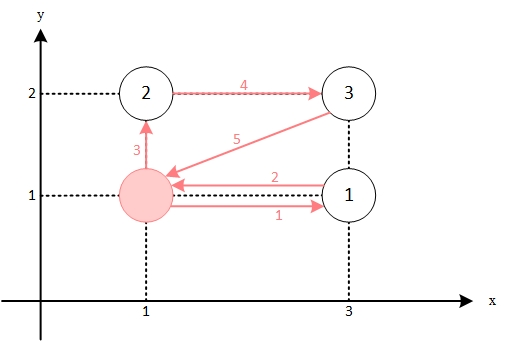
\includegraphics[width=0.5\linewidth]{picture/huawei_0904_3_1_output_interpretation}
	\captionsetup{font=scriptsize}
\end{figure}
红色箭头为最短距离的规划路径,顺序为图中红色序号,如图红色箭头5为客户3直达到公司。

\noindent\textbf{样例输入2:}

\lstset{numbers=none}
\begin{lstlisting}
4 1
2 2
1 1 1
1 3 4
3 1 2
3 3 3
\end{lstlisting}
\lstset{numbers=left}

\noindent\textbf{样例输出2:}
\lstset{numbers=none}
\begin{lstlisting}
11.3
\end{lstlisting}
\lstset{numbers=left}
维修工背包容量是1,逐个按优先级为每个客户更换设备,到每个客户单程距离计算为$\sqrt{2}$,往返一个客户距离是$2\sqrt{2}$,总路程为$8\sqrt{2}$,最短总距离四舍五入后为11.3。
	
\vspace{10pt}
	
\noindent\textbf{思路分析:}
\begin{itemize}
	\item [1.] \textbf{客户的优先级排序} 
	
	因为每个客户有不同的优先级(level),题目要求维护工根据客户优先级的顺序服务。所以在计算最短路径之前,我们首先要对客户按优先级进行排序。优先级排序后,维护工可以根据顺序为客户提供服务,这也是问题中的一个要求。
	
	\item [2.] \textbf{距离计算}
	
	维护工需要计算每次从公司出发到某个客户的距离,以及客户之间的距离。
	
	\begin{equation*}
		\begin{aligned}
			\mathcal{D} = \sqrt{(x_1 - x_2)^2 + (y_1 - y_2)^2}
		\end{aligned}
		\label{eq: Euclidean distance}
	\end{equation*}	
	
	\item[3.] \textbf{动态规划解决方案}
	\begin{itemize}
		\item [$\bullet$] \texttt{dp[i]} 表示服务前 i 个客户的最小总距离。
		
		\item [$\bullet$] 每次服务客户时,维护工最多可以携带 k 台设备。
	\end{itemize}
	
	\item[4.] \textbf{路径枚举}
	\begin{itemize}
		\item[$\bullet$] 维护工最多一次可以为 k 个客户服务。我们通过枚举每个客户服务顺序,尝试每一条可能的路径,计算其距离并更新 \texttt{dp} 表。
		
		\item[$\bullet$] 路径计算的过程包括:
			\begin{itemize}
				\item[1)] 从公司出发到第一个客户的距离。
				\item[2)] 客户之间的距离。
				\item[3)] 服务完最后一个客户后返回公司的距离。
			\end{itemize}
	\end{itemize}
	
\end{itemize}

\noindent\textbf{代码实现:}

1. \textbf{首先我们定义用户结构体 \texttt{Customer}}:
\begin{lstlisting}
struct Customer {
	int x;
	int y;
	int level;
};
\end{lstlisting}
\texttt{Customer} 结构体用于存储每个客户的坐标和优先级

2. \textbf{计算两点间距离的函数}
\begin{lstlisting}
double distance(int x1, int y1, int x2, int y2) { 
	double res;
	res = sqrt((x1 - x2) * (x1 - x2) + (y1 - y2) * (y1 - y2));
	return res;
}
\end{lstlisting}

3. \textbf{计算最小距离的核心函数}

1) 首先,我们对客户按 level 进行排序,以便优先为优先级较高的客户服务。
\begin{lstlisting}
// Sort customers by priority (level)
sort(customers.begin(), customers.end(), [](Customer a, Customer b) {
	return a.level < b.level;
});
\end{lstlisting}

2) 使用\texttt{dp[i]}用于存储前 i 个客户的最小距离
\begin{lstlisting}
// dp[i] represents the minimum total distance to serve the first i customers
vector<double> dp(n + 1, numeric_limits<double>::max());
dp[0] = 0.0; // Base case: no customers served yet, distance is 0
\end{lstlisting}

3) 预先计算了从公司到每个客户以及客户之间的所有距离。为了避免重复计算,加快后续的动态规划过程。
	\begin{itemize}
		\item[i] 计算公司到每个客户的距离
		
		\item[ii] 计算客户之间的距离 
	\end{itemize}
	
\begin{lstlisting}
// Precompute distances from the company to each customer and between customers
vector<vector<double>> dist(n + 1, vector<double>(n + 1));
for (int i = 0; i < n; ++i) { 
	dist[0][i + 1] = distance(company_x, company_y, customers[i].x, customers[i].y);
	dist[i + 1][0] = dist[0][i + 1]; // Return to company
	for (int j = 0; j < n; ++j) { 
		dist[i + 1][j + 1] = distance(customers[i].x, customers[i].y, customers[j].x, customers[j].y);
	}
}
\end{lstlisting}

4) 遍历每个可能的路径组合,计算从公司出发服务客户的最短距离。每次更新 \texttt{dp}表,确保其存储的是最短的路径总距离。
	
	\begin{itemize}
		\item[i] 外层循环 \texttt{for (int i = 0; i < n; ++i)} 枚举每个客户 \texttt{i} 作为本次服务的起点,也就是说从公司出发后先服务客户 \texttt{i}。
		
		\item[ii] 内层循环 \texttt{for (int j = i; j < n; ++j)} 从客户 \texttt{i} 开始,尝试服务 \texttt{i} 到 \texttt{j} 的客户组(最多 \texttt{k} 个客户),如果客户数量不超过 \texttt{k},则计算这段路径的总距离。
		
		\item[iii] 累加路径距离:首先计算从公司到第 \texttt{i} 个客户的距离 \texttt{dist[0][i + 1]},然后依次累加从 \texttt{i} 到 \texttt{j} 之间的客户的距离,最后再加上从第 \texttt{j} 个客户返回公司的距离。
		
		\item[iv] 更新 \texttt{dp} 表:对于每次找到的有效客户组合 \texttt{[i, j]},我们更新 \texttt{dp[j + 1]},表示服务完前 \texttt{j+1} 个客户后,所走的最短总距离。
	\end{itemize}

\begin{lstlisting}
// 暴力枚举
for (int i = 0; i < n; ++i) { 
	for (int j = i; j < n; ++j) {   
		// 计算服务的客户数量
		int num_customers = j - i + 1; 
		// 如果这组客户数量 <= k,才能被维护工一次性处理
		if (num_customers <= k) {
			// 从公司到第i个客户的距离
			double current_dist = dp[i] + dist[0][i + 1];
			
			for (int p = i; p < j; ++p) { 
				current_dist += dist[p + 1][p + 2]; // 客户之间的距离
			}
			
			// 从第 j 个客户返回公司
			current_dist += dist[j + 1][0];
			
			// 更新dp[j+1],即服务完前j+1个客户的最短距离
			dp[j + 1] = min(dp[j + 1], current_dist); 
		}
	}
}
\end{lstlisting}

\noindent\textbf{完整代码:}
	
\begin{lstlisting}
#include <iostream>
#include <vector>
#include <cmath>
#include <algorithm>
#include <limits>

using namespace std;

struct Customer {
	int x;
	int y;
	int level;
};

// Function to calculate the Euclidean distance between two points
double distance(int x1, int y1, int x2, int y2) { 
	double res;
	res = sqrt((x1 - x2) * (x1 - x2) + (y1 - y2) * (y1 - y2));
	return res;
}

// Enumeration method to find the minimum total distance
double calculate_min_distance(int n, int k, int company_x, int company_y, vector<Customer>& customers) { 
	// Sort customers by priority (level)
	sort(customers.begin(), customers.end(), [](Customer a, Customer b) {
		return a.level < b.level;
	});
	
	// dp[i] represents the minimum total distance to serve the first i customers
	vector<double> dp(n + 1, numeric_limits<double>::max());
	dp[0] = 0.0; // Base case: nno customers served yet, distance is 0
	
	// Precompute distances from the company to each customer and between customers
	vector<vector<double>> dist(n + 1, vector<double>(n + 1));
	for (int i = 0; i < n; ++i) { 
		dist[0][i + 1] = distance(company_x, company_y, customers[i].x, customers[i].y);
		dist[i + 1][0] = dist[0][i + 1]; // Return to company
		for (int j = 0; j < n; ++j) { 
			dist[i + 1][j + 1] = distance(customers[i].x, customers[i].y, customers[j].x, customers[j].y);
		}
	}
	
	// Enumerate all paths, trying every valid group of customers
	for (int i = 0; i < n; ++i) { 
		for (int j = i; j < n; ++j) { 
			int num_customers = j - i + 1;
			if (num_customers <= k) { // We can serve up to 'k' customers before returning to the company
				double current_dist = dp[i] + dist[0][i + 1]; // Distance to serve the first 'i' customers
				for (int p = i; p < j; ++p) { 
					current_dist += dist[p + 1][p + 2]; // Distance between customers
				}
				current_dist += dist[j + 1][0]; // Return to the company after serving the last customer
				dp[j + 1] = min(dp[j + 1], current_dist); // Update the minimum distance
			}
		}
	}
	
	return dp[n];
}

int main() {
	int n, k;
	cin >> n >> k;
	
	int company_x, company_y;
	cin >> company_x >> company_y;
	
	vector<Customer> customers(n);
	for (int i = 0; i < n; ++i) { 
		cin >> customers[i].x >> customers[i].y >> customers[i].level;
	}
	
	double result = calculate_min_distance(n, k, company_x, company_y, customers);
	printf("%.1f\n", result);
	
	return 0;
}
\end{lstlisting}

\end{document}